\chapter{Разработка приложения}
\label{cha:impl}

\section{Подготовка рабочего окружения}

Такой прогрессивный фреймворк, как Vue.js, очень легко интегрировать в проект: достаточно просто добавить на страницу JavaScript-файл и подключить его тегом \texttt{<script>}. Однако при создании крупных приложений рекомендуется использовать более продвинутые инструменты разработки, такие как пакетный менеджер \textbf{npm} \cite{npm} и компилятор JavaScript-кода \textbf{Babel} \cite{babel}.

\subsection{Менеджер пакетов npm}
Данный пакетный менеджер входит в состав программной платформы Node.js \cite{nodejs}. Главное преимущество npm в том, что его использование упрощает работу с модулями, необходимыми для работоспособности приложения, и производит их установку одной командой.

«Сердцевиной» любого приложения с модулями является файл \texttt{package.json}, который автоматически добавляется в папку с проектом при установке какого-либо пакета. Этот файл содержит в себе всю информацию о разрабатываемом приложении: наименование проекта, его автор, версия и описание, а также различные зависимости, указывающие на названия и версии пакетов, необходимых для работы приложения. В листинге \ref{lst:json} показана часть содержимого этого файла для разрабатываемого приложения.

\subsection{Транспилятор Babel}
\textbf{Babel}~--- это инструмент, который позволяет \textit{транспилировать} код, т.~е. выполнять преобразование современного кода в более ранний стандарт. Проблема заключается в поддержке браузерами различных версий JavaScript: не каждый браузерный движок полностью поддерживает стандарты ES7 и новее \cite{ecma}. По этой причине применение транспилера позволяет разработчикам использовать новейшие возможности языка JavaScript и не терять при этом совместимости со старыми движками браузеров.

\lstinputlisting[
caption=Файл package.json,
label=lst:json]
{listings/package.json}

\section{Клиентская часть приложения}

\subsection{Структура проекта}

Структура проекта в общем виде подробно описана на рис.~\ref{list:struct}. Все ресурсы и исходный код клиентской части веб-приложения находятся в директории \textit{src}.

\begin{figure}
	\dirtree{%
		.1 linguium/.
		.2 node-modules/
		\dotfill
		\begin{minipage}[t]{8cm}
			установленные пакеты npm
		\end{minipage}.
		.2 src/
		\dotfill
		\begin{minipage}[t]{8cm}
			исходные файлы проекта
		\end{minipage}.
		.3 assets/
		\dotfill
		\begin{minipage}[t]{8cm}
			статические ресурсы проекта
		\end{minipage}.
		.3 components/
		\dotfill
		\begin{minipage}[t]{8cm}
			все компоненты проекта
		\end{minipage}.
		.4 auth/
		\dotfill
		\begin{minipage}[t]{8cm}
			компоненты, отвечающие за авторизацию и аутентификацию
		\end{minipage}.
		.4 books/
		\dotfill
		\begin{minipage}[t]{8cm}
			компоненты, отвечающие за книги и их части
		\end{minipage}.
		.4 profile/
		\dotfill
		\begin{minipage}[t]{8cm}
			компоненты, отвечающие за профиль пользователя и его данные
		\end{minipage}.
		.4 ui/
		\dotfill
		\begin{minipage}[t]{8cm}
			компоненты, отвечающие за пользовательский интерфейс
		\end{minipage}.
		.4 ....
		.3 config/
		\dotfill
		\begin{minipage}[t]{8cm}
			конфиги: API яндекса и firebase
		\end{minipage}.
		.3 router/
		\dotfill
		\begin{minipage}[t]{8cm}
			роутер проекта
		\end{minipage}.
		.3 store/
		\dotfill
		\begin{minipage}[t]{8cm}
			папка с модулями хранилища Vuex
		\end{minipage}.
		.3 App.vue
		\dotfill
		\begin{minipage}[t]{8cm}
			корневой компонент проекта
		\end{minipage}.
		.3 main.js
		\dotfill
		\begin{minipage}[t]{8cm}
			точка входа приложения
		\end{minipage}.
		.3 ....
		.2 index.html
		\dotfill
		\begin{minipage}[t]{8cm}
			корневой HTML-шаблон
		\end{minipage}.
		.2 package.json
		\dotfill
		\begin{minipage}[t]{8cm}
			основная информация о проекте и его список зависимостей
		\end{minipage}.
		.2 ....
	} 
	\caption{Структура проекта}
	\label{list:struct}
\end{figure}

\subsection{Глобальное хранилище данных}

\textbf{Vuex}~--- это библиотека для управления состоянием, которая создает глобальное хранилище данных, доступное для всех компонентов приложения, в которых состояние может быть изменено исключительно предсказуемым образом.

Крупные приложения обычно состоят из большого числа компонентов, которые часто подлежат переиспользованию, и обмен данными между ними становится трудно отслеживать. Благодаря хранилищу все состояние приложения может быть представлено в одном месте, что делает приложение более организованным.

Vuex реализует подход к управлению состоянием, основанный на однонаправленном потоке данных. Его простейший вид представлен на рис.~\ref{fig:vuex}.

\begin{figure}
	\centering
	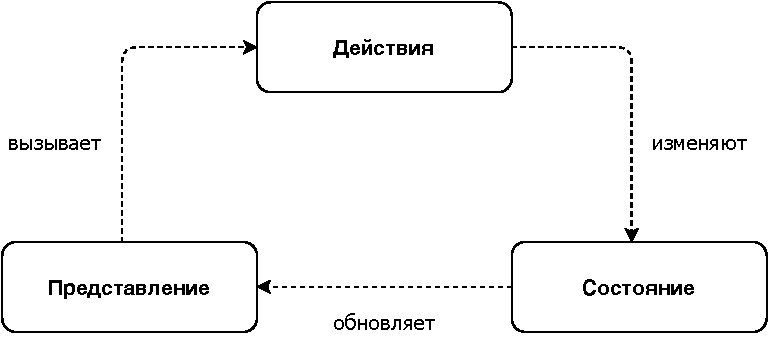
\includegraphics[width=0.9\textwidth, keepaspectratio]{figures/vuex}
	\caption{Однонаправленный поток данных}
	\label{fig:vuex}
\end{figure}

Однако для нескольких компонентов, зависящих от одного и того же состояния, описанный на рис.~\ref{fig:vuex} подход не работает. Данная проблема решается следующим образом: сперва вводится понятие общего состояния всего приложения, которое изменяется с помощью синхронных транзакций~--- \textbf{мутаций} (англ. \textit{mutations}). Мутации в свою очередь выполняются в ответ на асинхронную операцию~--- \textbf{действие} (англ. \textit{action}). И, наконец, действие инициирует мутацию через \textbf{диспетчер} (англ. \textit{dispatcher}).

Обновленная схема организации однонаправленного потока данных с использованием Vuex изображена на рис.~\ref{fig:vuex2}.

\begin{figure}
	\centering
	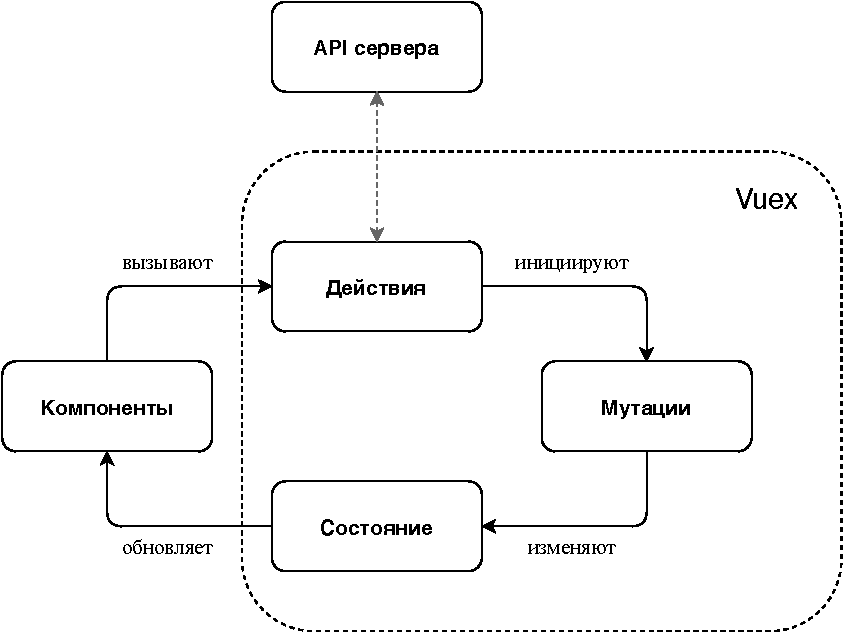
\includegraphics[width=0.95\textwidth, keepaspectratio]{figures/vuex2}
	\caption{Однонаправленный поток данных с Vuex}
	\label{fig:vuex2}
\end{figure}

При данном подходе дерево компонентов становится одним большим <<представлением>>, и любой компонент всегда сможет получить доступ к состоянию приложения или вызывать действие для изменения состояния. Таким образом подчеркивается независимость между представлением и состоянием, а также обеспечивается хорошая структурированность всего приложения и облегчение его отладки.

По умолчанию глобальные данные о состоянии всего приложения хранятся в одном объекте, в результате чего возникают проблемы со структурой данного объекта. По этой причине принято разделять хранилище на \textit{модули}, каждый из которых содержит независимые блоки глобального состояния, в которых есть свои собственные локальные мутации, действия и т.~п. Это также решает возможные проблемы с именованием, т.~к. у каждого модуля будет собственное пространство имен.

Хранилище, используемое в разрабатываемом приложении, было разделено на следующие модули:

\begin{itemize}
	\item информация о всех доступных книгах и их частях (модуль \textit{books});
	\item состояние текущего пользователя и доступные ему операции: авторизация, аутентификация, выход из учетной записи, изменение собственных данных и т. п. (модуль \textit{user});
	\item информация обо всех зарегистрированных учетных записях: имя, электронная почта и аватар каждого пользователя (модуль \textit{users});
	\item все статьи, написанные пользователями, и комментарии к этим статьям: возможность создавать, редактировать и удалять данные (модуль \textit{articles});
	\item система форума, состоящая из пользовательских тредов: функционал тот же, что и в модуле \textit{articles} (модуль \textit{forum});
	\item пользовательские данные: информация о всех прочитанных частях книг (момент времени, в который пользователь последний раз открывал ту или иную часть или же прочитал ее), а также информация о всех пользовательских словах, добавленных в процессе чтения, и все доступные операции над ними (модуль \textit{userdata}).
\end{itemize}

В качестве примера рассмотрим модуль \textit{books}, представленный в листинге \ref{lst:books}. Дадим некоторые пояснения:

\begin{itemize}
	\item в объекте \texttt{state} хранится состояние, содержащее пустой массив под названием books, который вскоре будет заполнен объектами (книгами) с помощью действия \texttt{loadBooks};
	\item мутация \texttt{setBooks}, находящаяся в объекте mutations, производит изменение \texttt{state}, присваивая переданные книги свойству \texttt{state.books};
	\item объект \texttt{actions} содержит асинхронный метод \texttt{loadBooks}, который извлекает данные из базы и совершает мутацию \texttt{setBooks} посредством \texttt{commit};
	\item объект \texttt{getters} включает в себя вспомогательную функцию \texttt{books}, которая возвращает массив объектов (список книг) на основе состояния.
\end{itemize}

\lstinputlisting[
caption=Модуль хранилища books,
label=lst:books]
{listings/books.js}

\clearpage

Затем уже внутри самого компонента добавляется вычисляемое свойство, которое возвращает соответствующий геттер из хранилища. Это свойство впредь можно будет как угодно переиспользовать, например, чтобы отфильтровать список книг или подсчитать их количество. Для вызова действия используется функция \texttt{dispatch}.

Раз уж речь идет о Vuex, стоит упомянуть, как выглядит метод, отвечающий за имплементацию метода интервальных повторений. Логика его реализации находится в функции \texttt{processUserdataWord}, которая входит в состав модуля \textit{userdata} (листинг \ref{lst:leitner}). Работает данная функция следующим образом: если поступающее в качестве аргумента слово находится в пятой и последней коробке (англ. \textit{bucket}), то оно считается запомненным и удаляется из пользовательского словаря. В противном случае временной интервал его следующего повторения увеличится в два раза и оно переместится в следующую по счету коробку.

\lstinputlisting[
caption=Имплементация метода интервальных повторений,
label=lst:leitner]
{listings/leitner2.js}

\subsection{Реактивность}

При создании первоначального экземпляра Vue для каждого свойства автоматически создается пара \textit{геттер и сеттер}. Именно они являются причиной обновления DOM всякий раз, когда изменяются данные. С помощью этих реактивных функций Vue может отслеживать любое изменение в любом свойстве и автоматически отрисовывать эти изменения. Кроме того, они позволяют Vue отслеживать зависимости между свойствами данных.

Также у каждого экземпляра компонента есть связанный с ним \textit{экземпляр наблюдателя}, задача которого~--- помечать все затронутые при отрисовке компонента поля как зависимости. Другими словами, он отвечает за реагирование на изменения данных. При вызове сеттера поля, помеченного наблюдателем как зависимость, этот сеттер уведомляет наблюдателя, и тот инициирует повторную отрисовку компонента, после чего обновляется дерево виртуального DOM. Весь этот процесс отражен на рис.~\ref{fig:react}.

\begin{figure}[h]
	\centering
	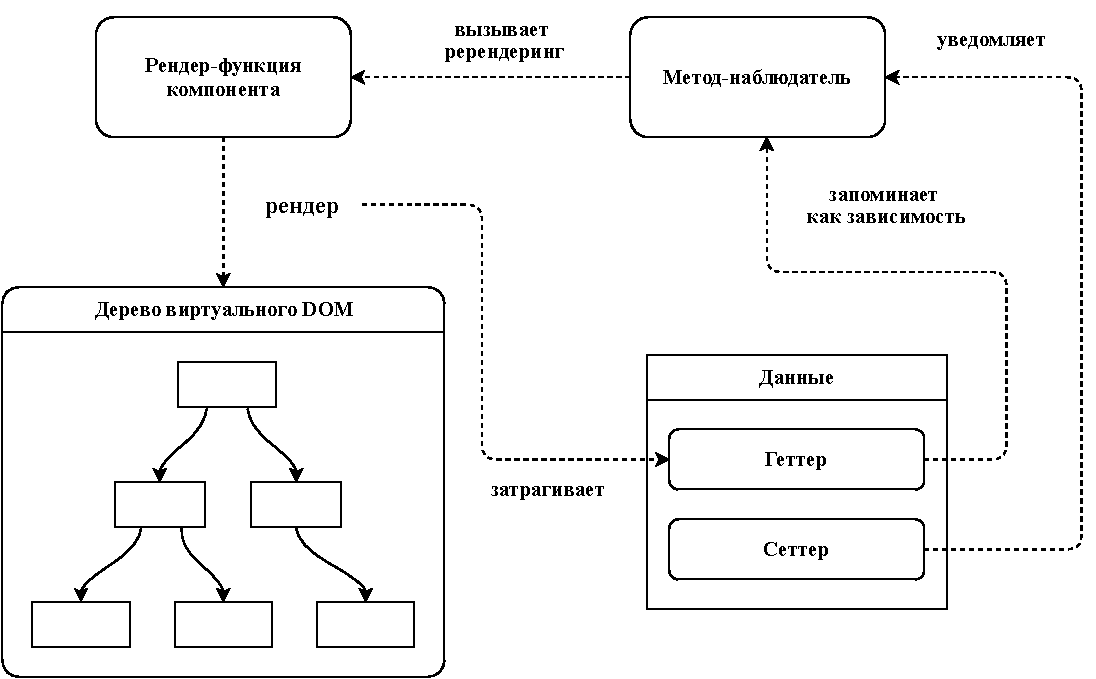
\includegraphics[width=\textwidth]{figures/reactivity}
	\caption{Визуализация работы реактивности}
	\label{fig:react}
\end{figure}

Однако у подобного способа отслеживания изменений имеется ряд особенностей и нюансов. Дело в том, что вследствие определенных ограничений JavaScript существуют такие виды изменений, которые Vue не способен обнаружить. К счастью, существуют способы обойти их и сохранить реактивность. Один из таких способов~--- метод \texttt{Vue.set}. Данный метод принимает на вход три аргумента:

\begin{itemize}
	\item объект, в который будет добавлено новое свойство;
	\item имя нового свойства либо его индекс;
	\item значение нового свойства.
\end{itemize}

Рассмотрим его на примере мутации \texttt{setUserName}, которая задает новое имя пользователя (листинг \ref{lst:vueset}). В данном случае новое свойство \texttt{name} добавляется в объект \texttt{state.user}, затем для этого свойства автоматически создается пара геттер и сеттер, которые обеспечивают его реактивность.

\lstinputlisting[
caption=Метод Vue.set,
label=lst:vueset]
{listings/vueset.txt}

\subsection{SpeechSynthesis}

Интерфейс \texttt{SpeechSynthesis} входит в состав Web Speech API и позволяет веб-приложению управлять голосовыми данными. Данная технология хоть и является экспериментальной, но уже поддерживается большинством браузеров \cite{speech}.

В разрабатываемом приложении \texttt{SpeechSynthesis} играет ключевую роль при изучении слов, ведь пользователю необходимо знать, как точно звучит слово, чтобы быть способным его произносить.

В листинге \ref{lst:speech} показаны две функции: \texttt{getVoices} для получения списка доступных голосов и функция \texttt{pronounceWord}, которая принимает на вход в качестве аргументов исходное слово для перевода и сам голос для его озвучивания.

\clearpage

\lstinputlisting[
caption=Получение списка голосов и произношение слова,
label=lst:speech]
{listings/speechSynthesis.js}

Метод \texttt{SpeechSynthesis.getVoices} возвращает список объектов \texttt{SpeechSynthesisVoice}, представляющих все доступные голоса.

Объект \texttt{SpeechSynthesisUtterance} содержит свойство текста, который будет синтезироваться при произнесении слова или высказывания, а также устанавливает определенные настройки по его звучанию (громкость, скорость, высота и голос озвучивания). Метод \texttt{SpeechSynthesis.speak} позволяет произносить полученную на вход информацию исходя из заданных настроек.

В листинге \ref{lst:words} показана инициализация \texttt{SpeechSynthesis} в компоненте. Для определенной выше в листинге \ref{lst:speech} функции \texttt{getVoices} применяется фильтр, который выбирает только английские голоса. Если хотя бы один такой голос доступен, то из этого массива голосов выбирается самый первый и кладется в переменную \texttt{voice} (сами голоса в основном различаются по полу и интонации говорящего). Для желаемого слова вызывается функция \texttt{pronounce}, которая вызывает определенный выше метод \texttt{pronounceWord} из листинга \ref{lst:speech} и озвучивает это слово заданным голосом.

\clearpage

\lstinputlisting[
caption=Инициализация SpeechSynthesis в компоненте,
label=lst:words]
{listings/userwords.vue}

\subsection{Axios}

\textbf{Axios}~--- это основанная на промисах библиотека для выполнения HTTP-запросов, которая позволяет получать и отображать данные из стороннего API.

С помощью Axios и API Яндекс.Переводчика \cite{yandex} становится возможна имплементация метода параллельного чтения, представленного в разделе 1. Синтаксис запроса для перевода текста представлен в листинге \ref{lst:yandex}. При инициализации запроса ответ возвращается в формате JSON. В таблице \ref{tab:tab2} приведено описание всех параметров, которые можно передать запросу, а в таблице \ref{tab:tab3} описаны возможные коды ответов.

\lstinputlisting[
caption=Синтаксис запроса Яндекс.Переводчика,
label=lst:yandex]
{listings/yandex.txt}

\begin{table}[h]
	\centering
	\begin{tabular}{ |c|l|c|c| }
		\hline
		Параметр & Описание \\
		\hline
		key & Бесплатный API-ключ \\
		\hline
		text & Текст, который необходимо перевести \\
		\hline
		lang & Направление перевода (например, \texttt{en-ru}) \\
		\hline
		format & Формат текста (текст без разметки или в формате HTML) \\
		\hline
		options & Опции перевода \\ 
		\hline
		callback & Имя функции обратного вызова \\ 
		\hline
	\end{tabular}
	\caption{Описание передаваемых параметров запросу}
	\label{tab:tab2}
\end{table}

\begin{table}[h]
	\centering
	\begin{tabular}{ |c|l|c|c| }
		\hline
		Значение & Описание \\
		\hline
		200 & Операция выполнена успешно \\
		\hline
		401 & Некорректный API-ключ \\
		\hline
		402 & API-ключ заблокирован \\
		\hline
		404 & Превышен суточный лимит на объем переведенного текста \\
		\hline
		413 & Превышен максимально допустимый размер текста \\ 
		\hline
		422 & Невозможно перевести текст \\ 
		\hline
		501 & Данное направление перевода не поддерживается \\ 
		\hline
	\end{tabular}
	\caption{Коды возможных ответов и их описание}
	\label{tab:tab3}
\end{table}

Имплементация метода параллельного чтения в компоненте показана в листинге \ref{lst:axios}. Он осуществляется засчет метода \texttt{window.getSelection}, который возвращает объект \texttt{Selection}, представленный в виде диапазона текста, который пользователь выделил на странице. Затем вызывается метод \texttt{getSelectedTextAndTranslate}, который осуществляет перевод выделенного текста с помощью вызова функции \texttt{getTranslation} и инициирует показ снэкбара с переводом текста.

В функции \texttt{getTranslation} осуществляется GET-запрос к API Яндекс.Переводчика с передаваемым ему фрагментом текста.

Яндекс.Переводчик использует гибридную модель машинного перевода, которая включает в себя нейросетевой и статистический подходы. Последний основан на моделях языка: исходный текст разбивается на слова и фразы, которые переводятся независимо друг от друга, после чего для каждой части текста подбирается потенциальный перевод из матрицы. Затем система выбирает лучший перевод с точки зрения сочетаемости слов в языке. Однако недостаток данного подхода в том, что не всегда удается установить взаимосвязь между фразами. И тут на помощь приходит нейросетевой подход, который позволяет учитывать контекст и добиться более связного по смыслу перевода. В отличие от статистического подхода, текст не разбивается на отдельные части, а переводится полностью. В данном подходе используется векторное представление слов (англ. \textit{word embedding}). Вектор состоит из чисел, которые характеризуют слово по семантическим и лексическим признакам. В итоге предложение представляет из себя векторное пространство, в котором нейронная сеть определяет семантику слов и взаимосвязь между ними.

Текст для перевода передается двум системам сразу, а затем на основе оценке алгоритма определяется, какой из переводов показывать пользователю. Таким образом, можно не беспокоиться о качестве перевода, т.~к. в большинстве случаев он будет относительно связным по смыслу.

\lstinputlisting[
caption=Имплементация метода параллельного чтения,
label=lst:axios]
{listings/axios.vue}

\subsection{Шина событий}

Рассмотрим такую ситуацию: пользователь решил изменить свой электронный адрес; для этого он зашел в настройки профиля, нажал на гипотетическую кнопку <<изменить>>~--- появилось модальное окно, в котором пользователь ввел новый адрес, который сервер успешно обработал. Проблема состоит в том, как же дать нашему приложению понять, в какой момент необходимо закрывать это модальное окно.

Для решения этой проблемы необходимо ввести такое понятие, как \textit{шина событий}. По сути, это экземпляр Vue, который используется для работы с событиями: он имеет возможность как имитировать события с помощью метода \texttt{\$emit}, так и подписываться на них благодаря методу \texttt{\$on} (рис.~\ref{fig:bus}).

\begin{figure}[h]
	\centering
	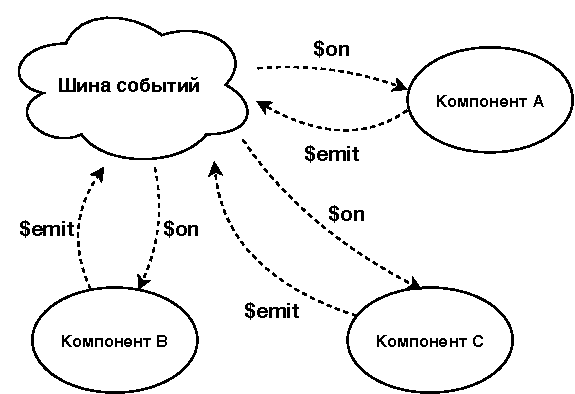
\includegraphics[width=0.85\textwidth, keepaspectratio]{figures/eventbus}
	\caption{Шина событий}
	\label{fig:bus}
\end{figure}

Создание шины событий отражено в листинге \ref{lst:bus1}. Метод \texttt{notify} можно назвать <<фасадом>> для функции \texttt{\$emit}, в то время как функция \texttt{setUpBus} на уровне прототипа Vue создает свойство \texttt{\$bus}, которое, являясь геттером, возвращает объект \texttt{EventBus}.

\clearpage

\lstinputlisting[
caption=Инициализация шины событий,
label=lst:bus1]
{listings/eventbus.js}

Затем в компоненте, который предназначен для изменения пользовательских данных и содержит в себе то самое незакрытое модальное окно, создадим хук \texttt{created}, в котором подпишемся на событие \texttt{useremail:changed}, а функциональность самого события будет заключаться в переключении значения переменной \texttt{userEmailDialog}; также для устранения утечки памяти стоит отписываться от события перед уничтожением экземпляра Vue, используя хуки \texttt{beforeDestroy} и метод \texttt{\$off} (листинг \ref{lst:bus2}).

Все, что осталось сделать,~--- имитировать это событие. События можно имитировать как из мутаций, так и напрямую из действий. В листинге \ref{lst:bus3} это делается через мутацию \texttt{setUserEmail}, отвечающую за изменение электронной почты пользователя. Теперь модальное окно закроется сразу как только имитируется данное событие.

Стоит отметить, что шина событий используется во многих частях разрабатываемого приложения: например, когда необходимо уведомить компонент об изменении состояния и отрисовать новое представление в ответ на определенный <<триггер>>.

\clearpage

\lstinputlisting[
caption=Подписка на событие в компоненте,
label=lst:bus2]
{listings/eventbus2.vue}

\lstinputlisting[
caption=Имитация события,
label=lst:bus3]
{listings/eventbus3.js}

\section{Серверная часть приложения}

\subsection{Структура базы данных}

Для хранения данных Cloud Firestore использует документы и коллекции. Если провести аналогию с системой управления баз данных реляционного типа (например, MySQL, PostgreSQL, Access, Oracle и т.~д.), то коллекция~--- это таблица, а документ является записью в этой таблице. Одна коллекция состоит из множества документов, которые содержат в себе набор полей или даже вложенные коллекции.

Структура всех коллекций базы данных для разрабатываемого приложения доступна в приложении А. С учетом того, что Cloud Firestore предоставляет возможность создания вложенных коллекций, следует уточнить, почему коллекция \textit{bookParts} (рис.~\ref{fig:bookPartsDiagram}) не была объявлена вложенной коллекцией для коллекции \textit{books} (рис.~\ref{fig:booksDiagram}). Дело в том, что при вызове одной коллекции также вызываются все ее вложенные коллекции, что неблагоприятно сказывается на оптимизации приложения. Таким образом, мы подсознательно идем на дубликацию некоторых данных, чтобы вытащить необходимые нам данные одним запросом. Учитывая то, что тарифный план Firebase имеет лимит на запросы для использования бесплатного режима (максимум 50 тыс. запросов на чтение в сутки), это является наиболее оптимальным и правильным решением.

\subsection{Правила базы данных}

Правила в Cloud Firestore обеспечивают контроль доступа к определенным коллекциям и документам и позволяют разработчику сосредоточиться на создании удобного пользовательского интерфейса без необходимости управления инфраструктурой или написания дополнительного кода на стороне сервера. 

Любое правило состоит из оператора \texttt{match}, которое идентифицирует документы в базе данных, а также из выражения \texttt{allow}, которое контролирует доступ к этим документам. Синтаксис для правила представлен в листинге \ref{lst:rule}.

\lstinputlisting[
caption=Синтаксис правила в Cloud Firestore,
label=lst:rule]
{listings/rule.txt}

Правила для разрабатываемого приложения представлены в листинге \ref{lst:rules}. Дадим некоторые пояснения:

\begin{itemize}
	\item функция \texttt{isSignedIn} определяет, авторизован ли пользователь;
	\item функция \texttt{isAdmin} определяет, является ли пользователь администратором веб-приложения;
	\item функция \texttt{isContentOwner} определяет, является ли пользователь автором заданного контента;
	\item любой документ из коллекции \textit{books} читать могут все пользователи, а писать в любой документ из данной коллекции имеет право только администратор;
	\item любой документ из коллекции \textit{articles} читать могут все пользователи, а писать в любой конкретно заданный документ из данной коллекции имеет право либо администратор, либо создатель документа;
	\item любой документ из коллекции \textit{forum} читать могут все пользователи, а писать в любой конкретно заданный документ из данной коллекции имеет право либо администратор, либо создатель документа;
	\item любой документ из коллекции \textit{users} читать могут все пользователи, а писать в любой конкретно заданный документ из данной коллекции имеет право либо администратор, либо конкретный пользователь с заданным уникальным идентификатором;
	\item любой документ из коллекции \textit{bookParts} читать могут только те пользователи, которые добавили их в свою пользовательскую коллекцию, а писать в любой документ из данной коллекции имеет право только администратор;
	\item любой документ из коллекции \textit{userdata} доступен для чтения и редактирования только для тех пользователей, чей уникальный идентификатор совпадает с именем документа.
\end{itemize}

Путь \verb|{document=**}|, который объявлен в некоторых правилах в листинге \ref{lst:rules}, соответствует любому документу в заданной коллекции. Оператор \texttt{read} определяет доступ к документу, а оператор \texttt{write} позволяет вносить изменения в заданный документ.

\clearpage

\lstinputlisting[
caption=Правила для разрабатываемого приложения,
label=lst:rules]
{listings/rules.txt}

\clearpage

\section{Вывод}

Результатом работы в рамках данного раздела является решение следующих задач:

\begin{itemize}
	\item было подготовлено окружение для разработки, которое позволило использовать актуальные на момент написания данного проекта технологии при создании веб-приложения;
	\item было создано адаптивное и соответствующее всем заявленным требованиям веб-приложение;
	\item были описаны основные модули приложения, а также детально изложена структура клиентской и серверной частей проекта.
\end{itemize}

%%% Local Variables:
%%% mode: latex
%%% TeX-master: "rpz"
%%% End:
